\subsection{Introduction} Face recognition systems have seen a great progress over the last several years with super-human recognition accuracy attainable in many scenarios. However, the accuracy of recognition degrades very significantly when dealing with very low resolution faces. In such conditions, the tasks of recognition and increasing the effective resolution (\textit{super-resolution}) become intertwined and necessitate joint solution. Indeed, developing  super-resolution techniques without regard for recognition often leads to face \textit{hallucination}, i.e.\ a process that creates plausibly looking faces lacking personal specifics. On the other hand, super-resolution has been known to benefit from recognition for a long time \cite{baker2002limits}.

\begin{figure}[t]
%\begin{wrapfigure}{i}{0.5\textwidth}
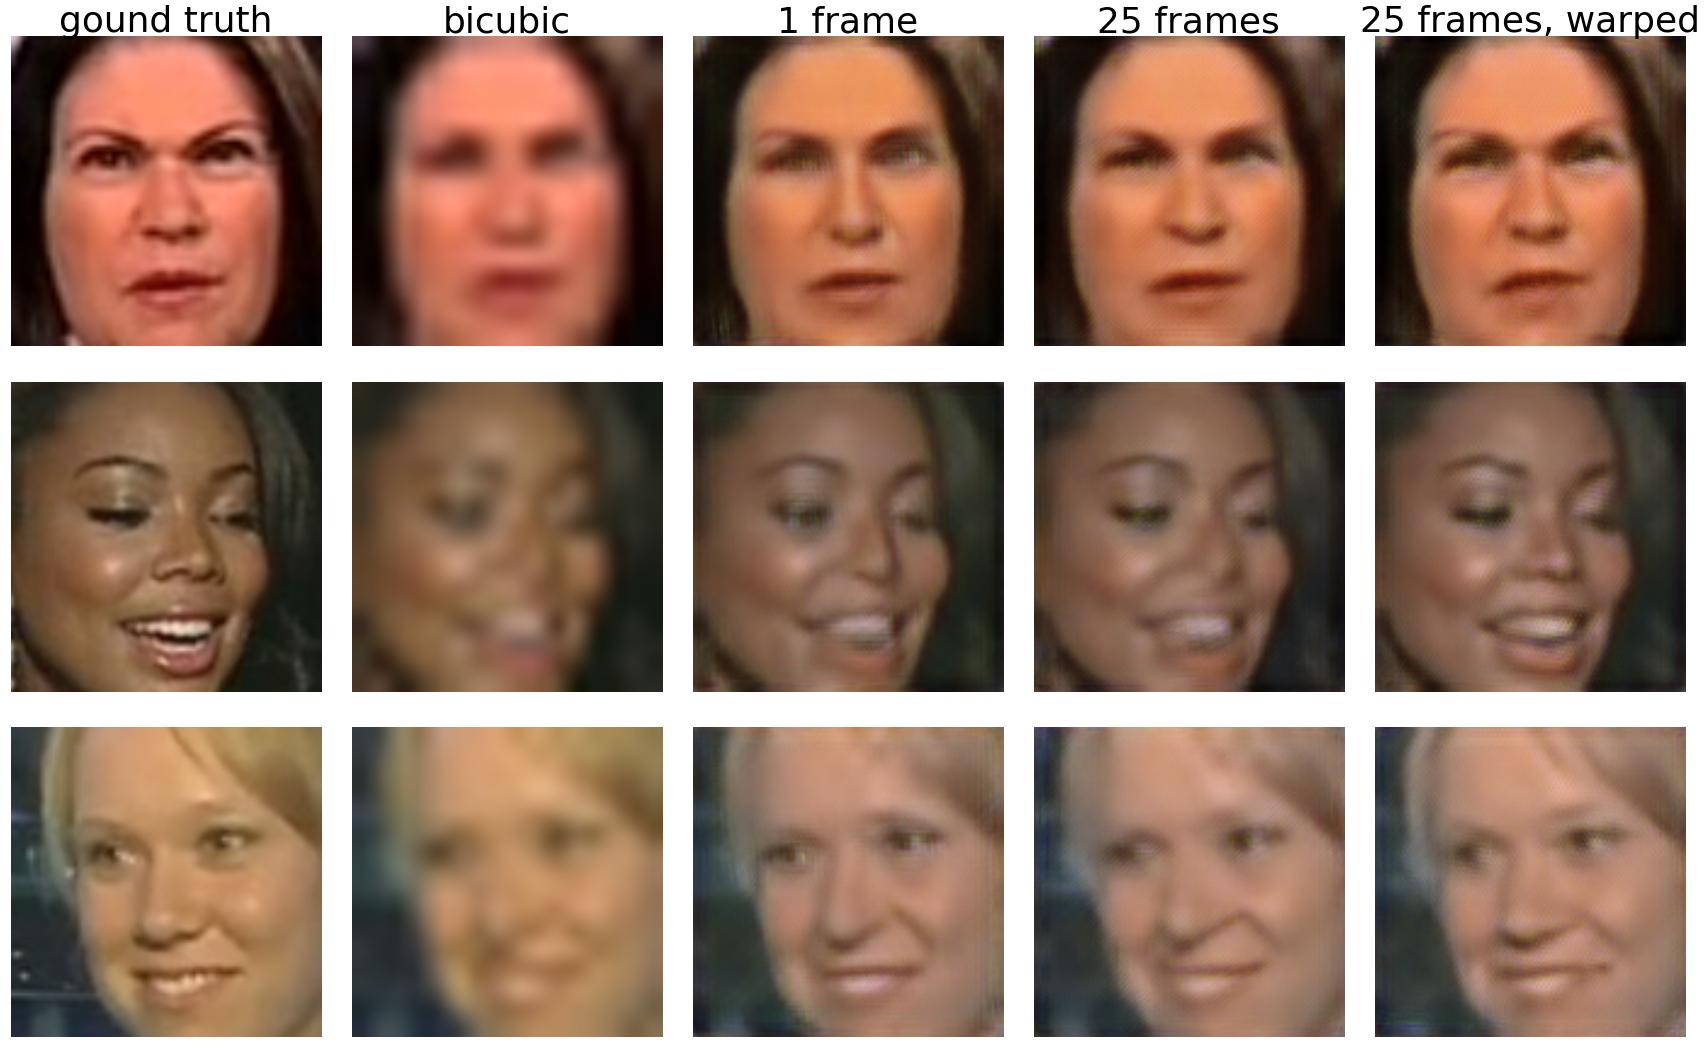
\includegraphics[width=\columnwidth]{\srroot/images/ytube/teaser.png}
\caption{Results of different super-resolution convolutional networks on samples from the Youtube Faces (YTF) dataset. From left to right: ground truth, bicubic upsampling,  single-frame superresolution, super-resolution from 25 frames without alignment (ours), super-resolution from 25 frames with warping subnetwork (ours).}
\label{fig:teaser}
%\vspace{10pt}
\end{figure}



While single-image super-resolution has recently drawn considerable attention \cite{ZhuLLT16, TuzelTH16}, super-resolution over large magnification factors can benefit significantly from information accumulated over multiple images, e.g.\ using adjacent frames in a surveillance stream or a video. Traditionally, multi-frame super-resolution has required rigid or non-rigid alignment with sub-pixel accuracy \cite{capel2003computer}. 
At the same time, faces have complex and deformable shapes leading to complex two-dimensional motion patterns which makes motion estimation hard to accomplish at sub-pixel precision. Generally, such precise alignment cannot be accomplished using low-level cues alone, and therefore requires high-level understanding/recognition of face geometry.



Motivated by all these observations, we present a system that performs multi-frame super-resolution by tackling all three inter-related problems, namely super-resolution, non-rigid alignment, and recognition, jointly and simultaneously. The tasks are implemented as modules of a deep neural network architecture that is trained in an end-to-end fashion on a dataset of realistic face videos \cite{WolfHM11}. The forward pass in our network involves pairwise alignment of pairs of frames performed in parallel with feature extraction, while the super-resolution is accomplished by a subsequent reconstruction module that takes warped features of the multiple frames into account. The learning process is driven by a combination of loss functions that includes the recognition-related loss ensuring that the super-resolution process reconstructs person-specific traits. 




%Here, we propose and evaluate a deep system that embraces all the aforementioned features: super-resolution, caring for recognition, multiple frames usage, motion recovering and avoiding hallucination. The system is trained end-to-end. \emph{Face Warping} sub-network is responsible for predicting the motion compensation transformation to align pairs of frames in a video-sequence to match one reference frame. The predicted transforms are applied to deep features of the frames in the input sequence, computed with \emph{Frame Feature extractors}. \emph{Combining} sub-network accepts all the transformed frames features and reconstructs the central frame in the sequence. 
Overall, while individual components of our system have been proposed in previous works, to the best of our knowledge, our work is the first that builds a systems that combines face super-resolution, recognition and alignment in a holistic manner. 
We evaluate the proposed architecture on the hold-out part of the YouTube Faces (YTF) dataset (\cite{WolfHM11}). We demonstrate good face verification  performance for the restored images using standard protocols adopted for the YTF dataset. We also show benefits of using multiple frames along with \emph{Face Warping} sub-network over the single-image approach. 
 We additionally compare our approach with  state-of-the-art face hallucination method \cite{ZhuLLT16} and find our method to perform better on the YouTube Faces dataset.

In the remainder of this work, we review the most related approaches in \ref{sec:related} describe the components of the proposed system in \ref{sec:video} and \ref{sec:loss} demonstrate the super-resolution results in \ref{sec:exps} and conclude with a short summary in \ref{sec:summary}. 
